\documentclass[11pt]{article}
\usepackage{graphicx}
\usepackage{amssymb,amsmath}
\usepackage[margin=2cm]{geometry}
\usepackage[colorlinks,bookmarksopen,bookmarksnumbered,citecolor=red,urlcolor=red]{hyperref}
\renewcommand{\vec}[1]{\boldsymbol{#1}}
\title{Quantum mechanical rotor}
\begin{document}
\maketitle
Throughout this document we use Hartree atomic units\footnote{\url{https://en.wikipedia.org/wiki/Hartree_atomic_units}} in which $\hbar=1$, distances are measured in units of $a_0=\frac{4\pi\epsilon_0\hbar^2}{m_e e^2}$, energies in units of $E_h=\frac{\hbar^2}{m_ea_0^2}$ and times in units of $\hbar/E_h$.
\section{Problem}
We consider the discretised action in \cite{Ammon2016} (see also \cite{Bietenholz1997})
\begin{equation}
S[\phi] = \frac{I}{a}\sum_{i=0}^{d-1} \left(
1-\cos(\phi_{i+1}-\phi_i)
\right)\label{eqn:action_discrete}
\end{equation}
for the state variable $\phi_i\in[-\pi,\pi)$ for $i=0,\dots,d-1$ with periodic boundery conditions. $I=M_0R^2$ is the angular moment and $a$ the lattice spacing. Since
\begin{equation}
\frac{1}{a^2}\left(1-\cos(\phi_{i+1}-\phi_i)\right) =
\frac{1}{2}\left(\frac{\phi_{i+1}-\phi_i}{a}\right)^2 + a^2 \left(
\frac{\phi_{i+1}-\phi_i}{a}\right)^4 + \mathcal{O}(a^4),
\end{equation}
Eq. \eqref{eqn:action_discrete} is a discretisation of the continuum action
\begin{equation*}
S_{\text{cont}}(\phi) = \frac{I}{2}\int_{0}^{T} \left(\frac{d\phi}{dt}\right)^2\;dt\qquad\text{with $T=a\cdot d$}
\end{equation*}
which naturally constrains the angle to $[-\pi,\pi)$.
\section{Fine-level sampling}
To generate the conditioned fine level sample at the odd sites, we need to sample from a distribution with the probability density
\begin{equation*}
p(\phi|\phi_+,\phi_-) = \mathcal{Z}^{-1}\exp\left[-\frac{I}{a}f(\phi;\phi_+,\phi_-)\right]
\end{equation*}
with
\begin{equation}
f(\phi;\phi_+,\phi_-) = 2-\cos(\phi_+-\phi)-\cos(\phi-\phi_-).
\label{eqn:f}
\end{equation}
where $\mathcal{Z}=\mathcal{Z}(\phi_+,\phi_-)$ is a normalisation constant.
We can now rewrite Eq. \eqref{eqn:f} as follows:
\begin{equation*}
\begin{aligned}
f(\phi;\phi_+,\phi_-) &= 2 - \cos(\phi_+)\cos(\phi)-\sin(\phi_+)\sin(\phi) - \cos(\phi_-)\cos(\phi)-\sin(\phi_-)\sin(\phi)\\
&= 2 - (\cos(\phi_+)+\cos(\phi_-))\cos(\phi) - (\sin(\phi_+)+\sin(\phi_-))\sin(\phi)\\
&= 2 - C \cos(\phi-\delta \phi)
\end{aligned}
\end{equation*}
for some constants $C=C(\phi_+,\phi_-)$ and $\delta\phi=\delta\phi(\phi_+,\phi_-)$. More specifically
\begin{xalignat*}{2}
\tan(\delta\phi) &= \frac{\sin(\phi_+)+\sin(\phi_-)}{\cos(\phi_+)+\cos(\phi_-)},&
C &= 2 \left|\cos\left(\frac{\phi_+-\phi_-}{2}\right)\right|.
\end{xalignat*}
Inserting this into Eq. \eqref{eqn:f} gives
\begin{equation*}
  f(\phi;\phi_+,\phi_-) = 2-C+2C\sin^2\left(\frac{\phi-\delta\phi}{2}\right).
\end{equation*}
Hence, the density we need to sample from can be written as
\begin{equation*}
p(\phi|\phi_+,\phi_-) = \tilde{\mathcal{Z}}^{-1}\exp\left[
-\frac{2IC}{a} \sin^2\left(\frac{\phi-\delta\phi}{2}\right)
\right].
\end{equation*}
Due to the obvious symmetries, it would be sufficient if we could sample from the density
\begin{equation}
p_\sigma(\psi) = \mathcal{Z}^{-1}_{\sigma} \exp\left[
-\sigma \sin^2\left(\frac{\psi}{2}\right)
\right]\qquad\text{for $\psi\in[-\pi,\pi]$ and $\sigma=\frac{2IC}{a}\ge 0$.}
\label{eqn:dist_psi}
\end{equation}
The normalisation constant $\mathcal{Z}_\sigma$ can be calculated by observing that
\begin{equation*}
  \mathcal{Z}_\sigma = \int_{-\pi}^{\pi} \exp\left[-\sigma\sin^2\left(\frac{\psi}{2}\right)\right] = 2\pi \exp\left[-\frac{\sigma}{2}\right]I_0\left(\frac{\sigma}{2}\right)
\end{equation*}
where $I_0$ is the modified Bessel function of the first kind. We might now sample approximately from the distribution in Eq. \eqref{eqn:dist_psi} by replacing $\sin^2(\psi/2)\mapsto \psi^2/4$ in the exponential, to obtain a Gaussian distribution with width $\sqrt{\frac{2}{\sigma}}$:
\begin{equation*}
  p_{\text{Gauss},\sigma} = \mathcal{Z}_{\text{Gauss},\sigma}^{-1} \exp\left[-\frac{\sigma}{4}\psi^2\right]\qquad\text{with $\mathcal{Z}_{\text{Gauss},\sigma}^{-1}=\sqrt{\frac{\sigma}{4\pi}}$}.
\end{equation*}
This is a good approximation if $\sigma$ is large (more specifically, $\sigma^{-1/2}\ll\pi$), but will not work so well for small value of $\sigma$, which can occur if $\phi_+-\phi_-\approx \pi$. Note that $\sigma\propto a^{-1}$, and hence for small lattice spacings $a$ Gaussian sampling is likely to become increasingly better (but we might still get some bad distributions from $\phi_+-\phi_-\approx\pi$).

Another possible solution is rejection sampling. For this, choose a number of points $\psi_i$, $i=0,\dots,M$ such that $\psi_0=0$, $\psi_M=\pi$ and construct the approximate, piecewise constant density
\begin{equation}
q_\sigma(\psi) = Z_{q,\sigma}^{-1} \exp\left[
-\sigma \sin^2\left(\frac{\psi_j}{2}\right)
\right]\qquad\text{for $\psi\in[\psi_{j},\psi_{j+1})$.}
\end{equation}
The normalisation constant can be calculated by observing that
\begin{equation*}
\sum_{j=0}^{M-1} (\psi_{j+1}-\psi_j) q_\sigma(\psi_j) = 1.
\end{equation*}
Since $\sin^2(\psi/2)$ is a montonously increasing function of $\psi$, we have that $p_\sigma(\psi)\le q_\sigma(\psi)$. Hence, rejection sampling would work like this:
\begin{enumerate}
\item Draw a sample $\hat{\psi}$ from $q_\sigma$. Since this is a piecewise constant distribution, this can be done very easily.
  \item Accept this sample with the probability $p_\sigma(\hat{\psi})/q_\sigma(\hat{\psi})$. Otherwise, continue with Step 1 (and repeat until a sample is accepted).
\end{enumerate}
The points $\psi_i$ should probably be chosen such that they are clustered closer together where the slope of $\sin^2(\psi/2)$ is large. This will ensure that the ratio $p_\sigma(\psi)/q_\sigma(\psi)$ is not too far from one, i.e. we accept as many points as possible.
\section{Continuum limit}
The Lagrangian of a free particle of mass $M_0$ constrained to a circle of radius $R$ is given by
\begin{equation}
\begin{aligned}
  \mathcal{L} &= \frac{M_0}{2}\left(\dot{x}^2+\dot{y}^2\right)\qquad\text{with $x^2+y^2=R^2$}\\
&= \frac{I}{2}\dot{\phi}^2=\frac{1}{2I} L^2 \qquad{\text{where $I:=R^2M_0$}}.
\end{aligned}
\label{eqn:Lagrangian_classical}
\end{equation}
Here we used the parametrisation $(x(t),y(t))=R(\cos(\phi(t)),\sin(\phi(t)))$ and the angular $L$ is defined as $L=I\dot{\phi}$. In the chosen units the time dependent Schr\"{o}dinger equation corresponding to the classical Lagrangian in Eq. \eqref{eqn:Lagrangian_classical} is obtained by replacing the angular momentum by an operator $\hat{L}$. However, as derived in \cite{Tanimura1994}, the Hilbert space $H$ is the sum of separate spaces $H_\theta$, each with a different vacuum angle $\theta\in[-\pi,\pi)$, in other words
  \begin{equation}
    H=\bigoplus_{\theta\in[-\pi,\pi)} H_\theta.
  \end{equation}
  The angular momentum operator is different on each of those spaces, in $H_\theta$ it becomes $\hat{L}=-i\partial_\phi-\frac{\theta}{2\pi}i$ and the corresponding Schr\"{o}dinger equation is
\begin{equation}
  -i\frac{\partial{\Psi(\phi,t)}}{\partial t} = H(\theta)\Psi(\phi,t)=-\frac{1}{2I} \left(\frac{\partial}{\partial \phi}-\frac{\theta}{2\pi}i\right)^2\Psi(\phi,t).\label{eqn:Schroedinger}
\end{equation}
Note that $\theta$ looks a lot like an external current. Making the ansatz
\begin{equation}
  \Psi(\phi,t) = \frac{1}{2\pi}\exp\left[-i(E_m(\theta)t-m\phi)\right]
\end{equation}
energy eigenvalues are
\begin{equation}
  E_m(\theta) = \frac{1}{2I}\left(m-\frac{\theta}{2\pi}\right)^2.
\end{equation}
The partition function at finite temperature $T$ is
\begin{equation}
  Z(\theta) = \operatorname{Tr}\;\exp\left[-TH(\theta)\right]
  = \sum_{m\in\mathbb{Z}} \exp\left[-\frac{T}{2I}\left(m-\frac{\theta}{2\pi}\right)^2\right].
\end{equation}
Since $Z(\theta+2\pi)=Z(\theta)$, it can be Fourier-expanded as
\begin{equation}
  Z(\theta)=\sum_{Q\in\mathbb{Z}} Z_Q e^{i\theta Q}.
\end{equation}
$Z_Q$ can be obtained by Fourier-transforming $Z(\theta)$ (see \cite{Bietenholz1997})
\begin{equation}
  Z_Q = \frac{1}{2\pi}\int_{-\pi}^{\pi} Z(\theta')e^{-i\theta'Q}d\theta'
  = \sqrt{\frac{2\pi^2}{T}}\exp\left[-\frac{2\pi^2I}{T}Q^2\right]
\end{equation}
The topological susceptibility is given by
\begin{equation}
  \begin{aligned}
    \mathbb{E}[\chi_t] &= -\frac{1}{T}\frac{\partial^2\log[Z(\theta)]}{\partial\theta^2}\Big\vert_{\theta=0}\\
    &= -\frac{1}{T}\frac{Z(\theta)(\partial^2_\theta Z(\theta))-(\partial_\theta Z(\theta))^2}{Z(\theta)^2}\Big\vert_{\theta=0}\\
    &= -\frac{1}{T}\frac{\partial^2_\theta Z(\theta)}{Z(\theta)}\Big\vert_{\theta=0}
    = \frac{1}{T}\frac{\sum_{Q\in\mathbb{Z}} Q^2 Z_Q}{\sum_{Q\in\mathbb{Z}}Z_Q}\\
    &= \frac{1}{T}\frac{\sum_{Q\in\mathbb{Z}} Q^2 \exp\left[-\frac{2\pi^2I}{T}Q^2\right]}{\sum_{Q\in\mathbb{Z}}\exp\left[-\frac{2\pi^2I}{T}Q^2\right]}\\
    &= \frac{1}{4\pi^2 I} S(z)\qquad\text{with $z:=\frac{4\pi^2 I}{T}$}
      \end{aligned}
\end{equation}
Where the function $S(z)=S_1(z)$ is defined by
\begin{equation}
  S_n(z) = z^n \frac{\sum_{Q^{2n}\in\mathbb{Z}}Q^2 \exp\left[-\frac{1}{2}zQ^2\right]}{\sum_{Q\in\mathbb{Z}}\exp\left[-\frac{1}{2}zQ^2\right]}\label{eqn:Sz}
\end{equation}
The variance of $\chi_t$ is given by
\begin{equation}
  \begin{aligned}
    \operatorname{Var}[\chi_t] &= \mathbb{E}\left[(\chi_t-\mathbb{E}[\chi_t])^2\right]=\mathbb{E}[\chi_t^2]-\mathbb{E}[\chi_t]^2\\
    &= \frac{1}{T^2}\frac{\sum_{Q\in\mathbb{Z}}Q^4\exp\left[-\frac{2\pi^2I}{T}Q^2\right]}{\sum_{Q\in\mathbb{Z}}\exp[-\frac{2\pi^2I}{T}Q^2]}-\mathbb{E}[\chi_t]^2\\
    &= \frac{1}{8\pi^4 I^2} R(z) \qquad\text{with $R(z):=\frac{S_2(z)-S_1(z)^2}{2}$.}
  \end{aligned}
\end{equation}
The functions $S(z)$ and $\tilde{S}(z)$ are visualised in Fig. \ref{fig:Splot}.
\begin{figure}
  \begin{center}
    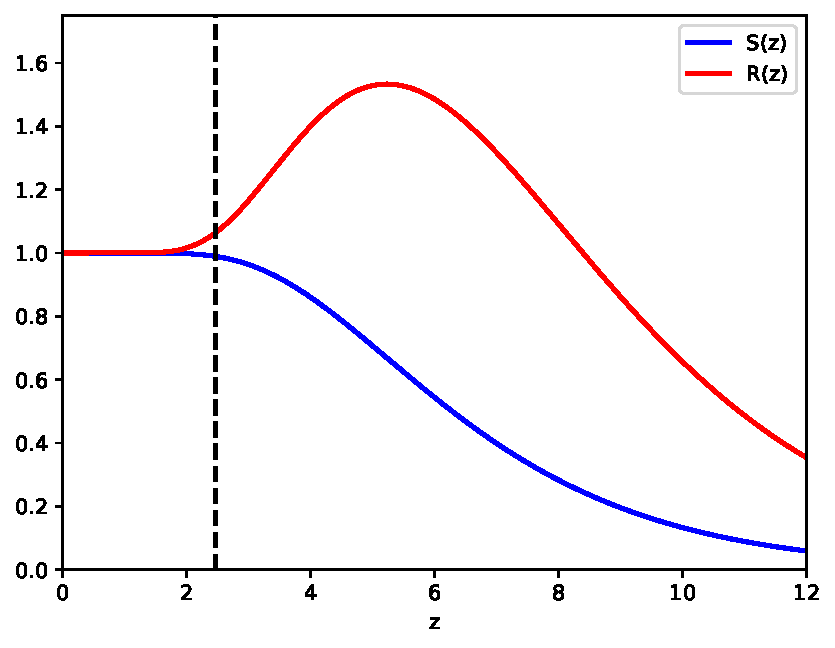
\includegraphics[width=0.5\linewidth]{SandR.pdf}
    \caption{Functions $S(z)$ and $R(z)$}
    \label{fig:Splot}
  \end{center}
\end{figure}
The infinite volume limit $T\rightarrow\infty$ corresponds to $z\rightarrow 0$, and for $z\ll 1$ the sums in Eq. \eqref{eqn:Sz} can be approximated by integrals (using $q=\sqrt{z}Q$) to obtain
\begin{equation}
  S_n(z) \approx \frac{\int_{-\infty}^\infty q^{2n} \exp\left[-\frac{1}{2}q^2\right]\;dq}{\int_{-\infty}^\infty \exp\left[-\frac{1}{2}q^2\right]\;dq}=(2n-1)!
\end{equation}
in particular $S(z)=S_1(z)\rightarrow 1$, $S_2(z)\rightarrow 3$ and $R(z)\rightarrow 1$.
\bibliographystyle{unsrt}
\bibliography{rotor}
\end{document}
